%!TEX root = ../../thesis.tex

\section{Earth's atmosphere, in the nIR}

While the Earth's atmosphere is important for life on Earth, it can be a nuisance for ground-based astronomical observations.
While the atmosphere is mostly transparent in the visible, with only minor transmission and emission features, it is not uniformly transparent in the infrared.

As light from astronomical sources passes through Earth's atmosphere, the molecular species absorb specific wavelengths (corresponding to molecular rotational and vibrational energy levels) densely populating the \nir{} with absorption lines, commonly referred to as telluric absorption.
\Cref{fig:croppedmolecfitabsorbtion} contains the model telluric absorption spectrum for the atmosphere from 0.3--30\um{} at $R\sim10\,000$ from~\citet{smette_molecfit_2015}.
It clearly shows that there are regions where the atmosphere is mostly transparent (transmission of 1), with other wavelength regions (e.g.\ at 4.5\um{}) that are completely opaque.
Molecules which are the main contributors to the absorption are labelled.

\begin{figure}
    \centering
    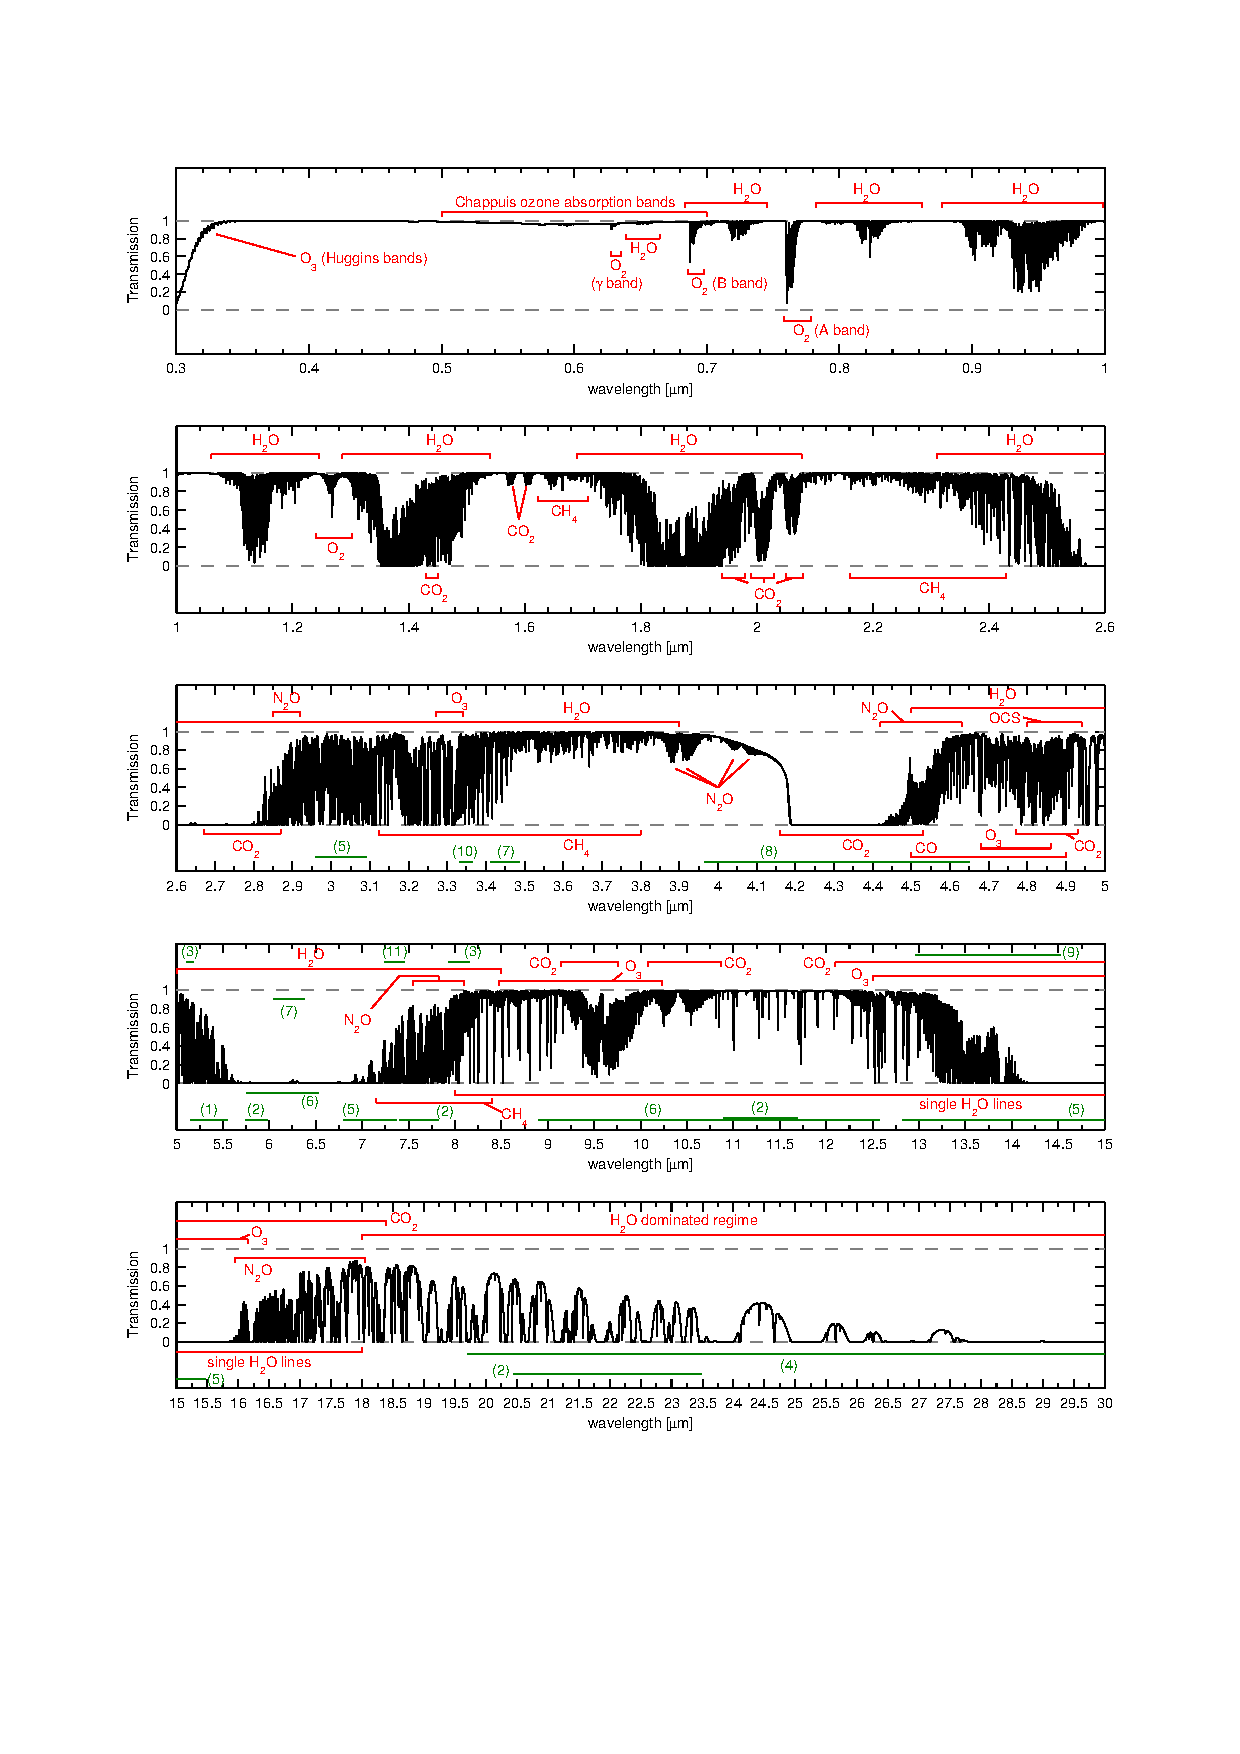
\includegraphics[width=0.9\linewidth]{figures/atmos_and_models/cropped_molecfit_absorption}
    \caption[Telluric absorption map from 0.3--30\um{} at $R\sim10\,000$.]{Telluric absorption map from 0.3--30\um{} at $R\sim10\,000$.
        The eight main molecules \ce{O2}, \ce{O3}, \ce{H2O}, \ce{CO}, \ce{CO2}, \ce{CH4}, \ce{OCS}, and \ce{N2O} contribute more than 5\% to the absorption in some wavelength regimes.
        The red regions mark the ranges where they mainly affect the transmission, minor contributions of these molecules are not shown.
        The green regions denote minor contributions from the following molecules: (1) \ce{NO}; (2) \ce{HNO3}; (3) \ce{COF2}; (4) \ce{H2O2}; (5) {HCN}; (6) \ce{NH3}; (7) \ce{NO2}; (8) \ce{N2}; (9) \ce{C2H2}; (10) \ce{C2H6}; and (11) \ce{SO2}.
        Credit~\citet[][Figure~1]{smette_molecfit_2015}.}
    \label{fig:croppedmolecfitabsorbtion}
\end{figure}

The windows of transmission defined the location of photometric bands in the infrared, with the common ones listed in \cref{tab:infrared_bands}~\citep[see e.g.][]{sterken_astronomical_1992, binney_galactic_1998}.
There are also variations on these bands for specific to different sites.
These photometric bands are chosen for high average photometric\footnote{Considering all photons in the band equally, regardless of wavelength (Very low resolution)} throughput, and do not consider the variable spectroscopic content inside the individual bands that becomes evident when observing at high resolution.

%!TEX root = ../../thesis.tex

\begin{table}
    \centering
    \caption{Standard infrared pass-bands.}
    \begin{tabular}{lcc}
        \toprule
        Band & Central wavelength [\um] & Bandwidth [\um]\\
        \midrule
        Z & 0.9  & 0.06 \\
        Y & 1.05 & 0.12 \\
        J & 1.25 & 0.38 \\
        H & 1.65 & 0.48 \\
        K & 2.2  & 0.4  \\
        L & 3.5  & 1.2  \\
        M & 4.8  & 0.6  \\
        N & 10.6 & 2.5  \\
        Q & 21   & 5.8  \\
        \bottomrule
    \end{tabular} \label{tab:infrared_bands}
\end{table}

The most prominent absorber in the infrared is water vapour (\ce{H2O}) which is a strong absorber and defines the photometric bands as seen in \cref{tab:infrared_bands}.
Water vapour is mostly concentrated in the lower 5\,\si{\kilo\metre}, so infrared observatories are situated in dry places at high altitude.
Even under ideal conditions the absorption of water vapour defines the IR bands.
Other molecular species in the atmosphere such as: \ce{CO}, \ce{CO2}, \ce{CH4}, are also important at various wavelengths.

When performing spectroscopy from the ground, the absorption spectrum of Earth's atmosphere contaminates the spectrum of the intended target.
In high-resolution spectroscopy the stellar and atmospheric lines can be resolved allowing for the identification and separation of the spectra.
The removal or correction for the telluric lines is very important for accurate science, especially for detecting exoplanet atmospheres in which the species trying to be detected also reside in the atmosphere~\citep{snellen_orbital_2010, brogi_carbon_2014, dekok_detection_2013}.

The absorption of atmosphere is highly variable on many different time scales.
The change in water vapour can occur rapidly over the course of the night while the concentrations of atmospheric constituents vary seasonally and even longer\footnote{For instance the increase in atmospheric \ce{CO2} caused by anthropamorphic climate change has caused a 6\% change to \ce{CO2} line depths since 2000~\citep{smette_molecfit_2015}.}.

On top of this is the observational dependence on the airmass of the target.
The airmass\footnote{Airmass $m=\sec{\theta}$ where $\theta$ is the zenith angle.} is the relative path length through the atmosphere compared to zenith.
The light of a target at a higher airmass passes through more of the atmosphere and is contaminated with deeper telluric lines.

Works such as~\citet{snellen_orbital_2010}, fit and remove the telluric variation during a series of continuous observations\footnote{51 spectrum of the same target in 180 minutes for~\citet{snellen_orbital_2010}}, to accurately remove the varying telluric lines and detect the absorption lines of exoplanet atmospheres.
